
\begin{frame}
DCM -> Direction Cosine Matrix (pre 3.2)
Transformation to inertial to body axes.
Quaternion 4 by 1
\end{frame}





  \begin{frame}[t]{Zmena súradníc}
\begin{itemize}
  \item<1-> aaaa
\end{itemize}

  \begin{onlyenv}<1->
  \begin{figure}
\centering
  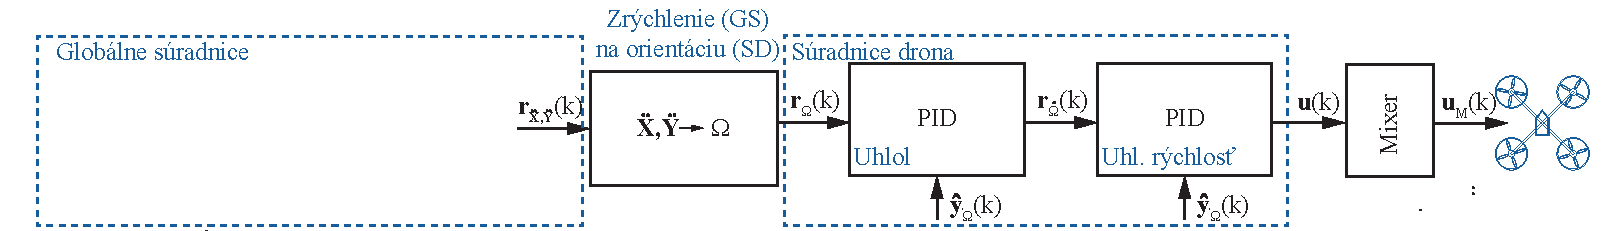
\includegraphics[width=\textwidth]{PID_HighLevel2}\\
\end{figure}
\end{onlyenv}

  \end{frame}



  \begin{frame}[t]{Rýchlosť}
\begin{itemize}
  \item<1->   \item<1-> Väčšinou je to PID riadenie, ako aj pri ArduCopter, PX4 a inde (c.f. \cite{Saha2020}).
\end{itemize}

  \begin{onlyenv}<1->
  \begin{figure}
\centering
  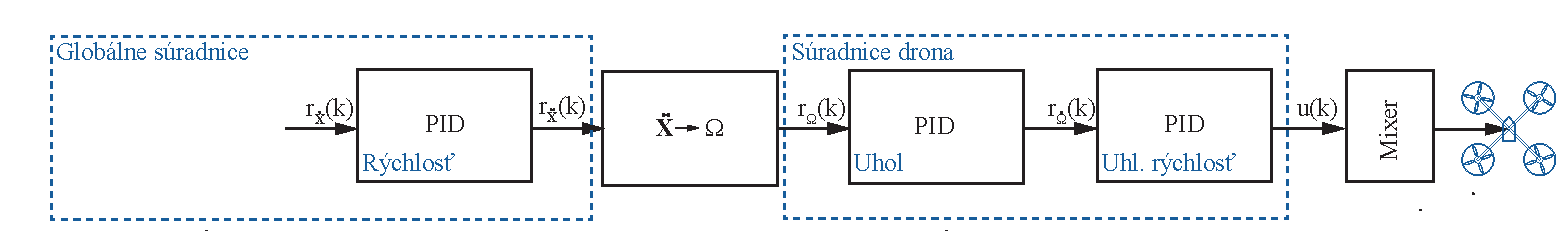
\includegraphics[width=\textwidth]{PID_HighLevel3}\\
\end{figure}
\end{onlyenv}


  \begin{onlyenv}<2->
  \begin{figure}
\centering
  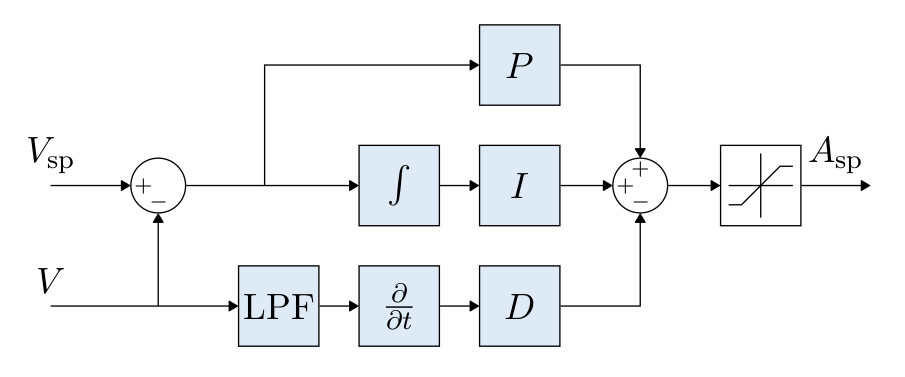
\includegraphics[width=70mm]{PX4_Velocity}\\
\end{figure}
\end{onlyenv}

  \end{frame}


 \begin{frame}[t]{Poloha}
\begin{itemize}
  \item<1-> Väčšinou je to P riadenie, ako aj pri ArduCopter, PX4 a inde (c.f. \cite{Saha2020}).
\end{itemize}

  \begin{onlyenv}<1->
  \begin{figure}
\centering
  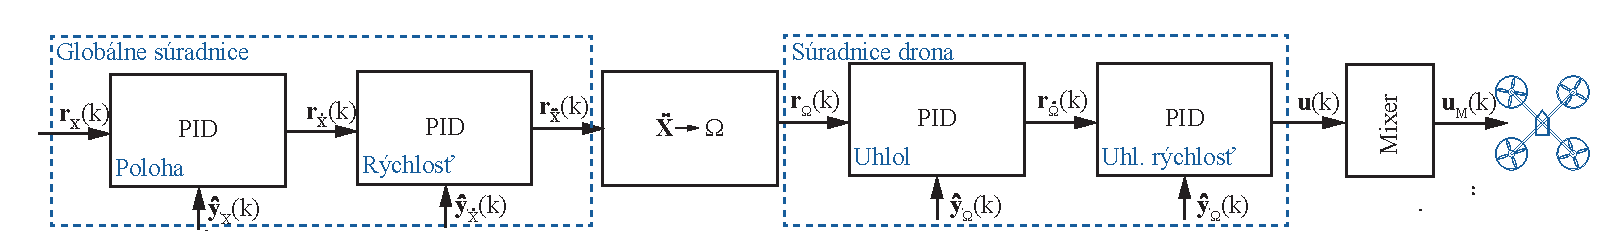
\includegraphics[width=\textwidth]{PID_HighLevel4}\\
\end{figure}
\end{onlyenv}


  \begin{onlyenv}<2->
  \begin{figure}
\centering
  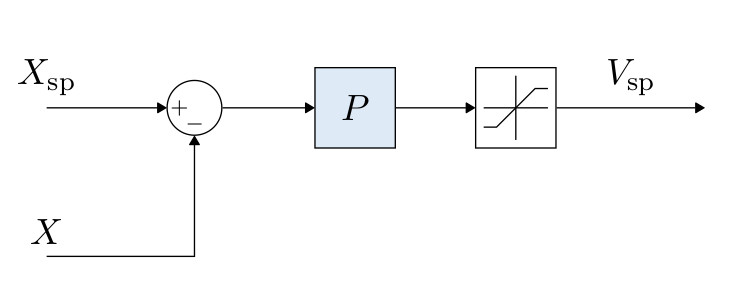
\includegraphics[width=50mm]{PX4_Position}\\
\end{figure}
\end{onlyenv}
  \end{frame}




\begin{frame}{Je perfektné sledovanie trasy možné?}
\begin{itemize}
\item<1-> Majme trasu WP1 do WP2, všetko je v poriadku.
\item<2-> Pridajme WP3 a rozmýšľajme čo sa deje pri WP2. Je možné preletieť nad WP2?
\item<3-> Buď musíme úplne sa zastaviť alebo nemôžeme priamo preletieť --- ináč by sme potrebovali nekonečne veľké zrýchlenia
\end{itemize}

\begin{onlyenv}<1>
  \begin{figure}
\centering
  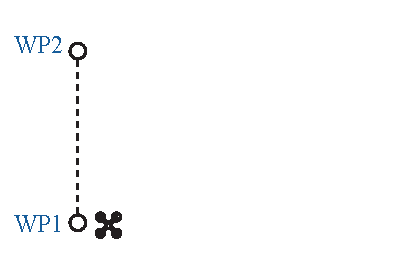
\includegraphics[width=60mm]{PositionControl}\\
\end{figure}
\end{onlyenv}

\begin{onlyenv}<2>
  \begin{figure}
\centering
  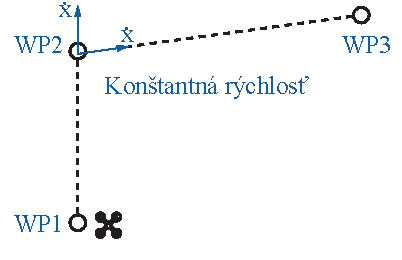
\includegraphics[width=60mm]{PositionControl2}\\
\end{figure}
\end{onlyenv}

\begin{onlyenv}<3>
  \begin{figure}
\centering
  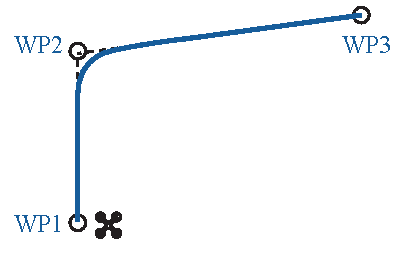
\includegraphics[width=60mm]{PositionControl3}\\
\end{figure}
\end{onlyenv}
\end{frame}
